\documentclass[../calc3.tex]{subfiles}
\graphicspath{{\subfix{../figures/}}}
\begin{document}
\chapter{Three-Dimensional Coordinate Systems}
\section{Vectors in the Plane}
The first goal for calculus 3 is to define the rectangular coordinate plane in 3-space.

In 2-space, this is the normal coordinate axis with coordinates $(x,y)$.

In 3-space, you now have $(x,y,z)$. We have an $xy$-plane, a $yz$-plane, and an $xz$-plane. Also we have octants in 3-space similar to quadrants in 2-space.

The $z$-axis is determined by the right-hand rule: if you curl the fingers on your right hand from the positive $x$-axis to the $y$-axis, your thumb points in the direction of the positive $z$-axis.

\ex Graph $(2,3,4)$.

When graphing points in 3-space, it might be easier to draw a prism to see the three-dimensional components easier.

\ex Graph $(-3,2,-6)$.

In 3-space the distance formula is simliar to 2-space. It is the following:
\[ d=\sqrt{(x_1-x_2)^2+(y_1-y_2)^2+(z_1-z_2)^2} \]

\begin{example}
    Find the distance between $(2,3,4)$ and $(-3,2,-6)$.

    Plug in the numbers into the formula and the answer gives $d=\sqrt{126}$
\end{example}

Similar to circles in 2-space, there are spheres in 3-space. The equation of a sphere is 
\[ (x-x_0)^2+(y-y_0)^2+(z-z_0)^2=r^2 \]

\begin{example}
    Write the equation of a sphere with a diameter having endpoints $(-1,2,1)$ and $(0,2,3)$.

    We can find the center with the midpoint formula, and the center is $(-\frac{1}{2},2,2)$.

    Using the $(-1,2,1)$ endpoint and the center calculated above, we can determine the radius to be $\sqrt{5/4}$.

    Therefore the equation of the sphere is $(x+\frac{1}{2})^2+(y-2)^2+(z-2)^2=\frac{5}{4}$.
\end{example}

\begin{example}
    Find the center and radius of the sphere $x^2+y^2+z^2-2x-4y+8z+17=0$.

    When we complete the square for this, we end up getting $(x-1)^2+(y-2)^2+(z+4)^2=4$.

    Therefore, the center is $(1,2,-4)$ and the radius is $2$.
\end{example}
\pagebreak
\begin{theorem}
    An equation of the form $x^2+y^2+z^2+Gx+Hy+Iz+J=0$ represents a sphere, a point, or has no graph.
\end{theorem}
We would get a point if the radius gives you 0, and if the radius is negative, then there is no graph.

\ex Graph $y=3$ in $\mathbb{R}^3$.

\ex Describe and sketch the surface in $\mathbb{R}^3$ represented by $y=x$.

\ex Graph $x^2+z^2=1$.

\begin{example}
    Describe the graph of $1\leq x^2+y^2+z^2\leq 4$. What if $z\leq 0$?

    This will represent the region between the spheres and centered at the origin with radii of $1$ and $2$. (This is a sphere with center cut out).
    
    The condition $z\leq 0$ will give us a hemisphere, it will only give the lower half of the figure.
\end{example}

\section{Vectors}
\begin{definition}[Vector]
    A vector indicates a quantity that has both magnitude and direction. 

    Examples include displacement, velocity, or force.
\end{definition}
Some ways to notate vectors are $\textbf{u}$, $\overrightarrow{u}$, $\vec{u}$, $\overrightarrow{AB}$, $\vec{AB}$. For the last two of these, these are read as a vector starting at $A$, heading towards $B$.

We say that 2 vectors are equivalent (or equal) if they have the same length and direction.

$0$ vector $(\textbf{0})$ has a length of $0$ and no direction. (Note that $\textbf{0}$ is a vector because it is bolded.)

\begin{definition}[Vector Addition]
    If $\textbf{u}$ and $\textbf{v}$ are positioned so that the initial point of $\textbf{v}$ is at the terminal point of $\textbf{u}$, then $\textbf{u}+\textbf{v}$ is the vector from the initial point of $\textbf{u}$ to the terminal point of $\textbf{v}$.
\end{definition}
Note that $\vec{u}+\vec{v}=\vec{v}+\vec{u}$.

\begin{definition}[Scalar Multiplication]
    If $c$ is a scalar and $\textbf{v}$ is a vector, then $c\textbf{v}$ is the vector whose length is $|c|$ times the length of $\textbf{v}$ and whose direction is the same as $\textbf{v}$ if $c>0$ and is opposite if $c<0$.
\end{definition}

Using the two definitions above, we can find the difference $\textbf{u}-\textbf{v}$. From the above definitions, we can rewrite this as $\vec{u}+(-\vec{v})$, which is equivalent to $\vec{u}-\vec{v}$.

\ex Sketch $\textbf{a}-2\textbf{b}$ and define $\textbf{a}$ and $\textbf{b}$ as you wish.

Coordinate Systems: Generally we place the initial point at the origin and then express a vector as $\textbf{a}=\langle a_1, a_2\rangle$ or $\textbf{a}=\langle a_1,a_2,a_3\rangle$ where $(a_1,a_2)$ 
and $(a_1,a_2,a_3)$ are terminal points.

Given points $A(x_1,y_1)$ and $B(x_2,y_2)$, vector $\textbf{a}=\textbf{AB}$ is $\textbf{a}=\langle x_2-x_1,y_2-y_1\rangle$. (In 3-space the idea is similar.)

\begin{example}
    Express vector $\overrightarrow{P_1P_2}$ in bracket notation if $P_1(1,3)$ and $P_2(4,-2)$.

    Note that we start at the terminal point. Therefore we have $\overrightarrow{P_1P_2}=\langle 4-1,-2-3\rangle=\langle 3,-5\rangle$.

    Note that the vector between the two points and the vector found have the same direction and same length.
\end{example}

Arithmetic Operations: If $\vec{v}=\langle v_1,v_2\rangle$ and $\vec{w}=\langle w_1,w_2\rangle$, then 
\begin{itemize}
    \item $\vec{v}+\vec{w}=\langle v_1+w_1,v_2+w_2\rangle$
    \item $\vec{v}-\vec{w}=\langle v_1-w_1,v_2-w_2\rangle$
    \item $k\vec{v}=\langle kv_1,kv_2\rangle$
\end{itemize}

\begin{example}
    If $\vec{a}=\langle -2,0,1\rangle$ and $\vec{b}=\langle 3,5,-4\rangle$, find $\vec{a}+\vec{b}$ and $\vec{b}-2\vec{a}$.

    Finding $\vec{a}+\vec{b}$ is simple just add them together to get $\langle 1,5,-3\rangle$.

    To find $\vec{b}-2\vec{a}$, multiply $\vec{a}$ by $2$ to get $\langle -4,0,2\rangle$. Then subtracting gives you $\langle 7,5,-6\rangle$.
\end{example}

Properties of Vectors:
\begin{enumerate}
    \item $\vec{a}+\vec{b}=\vec{b}+\vec{a}$
    \item $\vec{a}+(\vec{b}+\vec{c})=(\vec{a}+\vec{b})+\vec{c}$
    \item $\vec{a}+\textbf{0}=\vec{a}$
    \item $\vec{a}+(-\vec{a})=\textbf{0}$ (Additive Inverse)
    \item $c(\vec{a}+\vec{b})=c\vec{a}+c\vec{b}$
    \item $(c+d)\vec{a}=c\vec{a}+d\vec{a}$
    \item $(cd)\vec{a}=c(d\vec{a})$
    \item $1\vec{a}=\vec{a}$
\end{enumerate}

\begin{example}
    Prove property $\#2$ from above.

    Let $\vec{a}=\langle a_1,a_2\rangle$, $\vec{b}=\langle b_1,b_2\rangle$, and $\vec{c}=\langle c_1,c_2\rangle$.

    From the left side of property 2, we have $\langle a_1,a_2\rangle+(\langle b_1,b_2\rangle + \langle c_1,c_2\rangle)$.

    From this, we can simplify to get $\langle a_1+a_2\rangle + \langle b_1+c_1,b_2+c_2\rangle$.

    This gives us $\langle a_1+(b_1+c_1),a_2+(b_2+c_2)\rangle$.

    From the associative law we can rewrite this as $\langle (a_1+b_1)+c_1,(a_2+b_2)+c_2\rangle$.

    This is $\langle a_1+b_1,a_2+b_2\rangle + \langle c_1+c_2\rangle$, which is equivalent to $(\vec{a}+\vec{b})+\vec{c}$. \qed
\end{example}

Unit Vectors: A unit vector is a vector with a length of $1$.

In 2-space, define $\vec{i}=\textbf{i}=\langle 1,0\rangle$ and $\vec{j}=\textbf{j}=\langle 0,1\rangle$ and 3-space, $\vec{i}=\textbf{i}=\langle 1,0,0\rangle$, $\vec{j}=\textbf{j}
=\langle 0,1,0\rangle$, and $\vec{k}=\textbf{k}=\langle 0,0,1\rangle$.

$\vec{i},\vec{j}$, and $\vec{k}$ are called unit or standard basis vectors. All have length 1 and point in the positive direction on the $x-$,$y-$, and $z-$ axes.

For example, $\vec{a}=\langle 1,3,-4\rangle$ can be expressed as $\vec{a}=\vec{i}+3\vec{j}-4\vec{k}$.

\begin{example}
    If $\vec{a}=\vec{i}+2\vec{j}-3\vec{k}$, and $\vec{b}=4\vec{i}+7\vec{k}$, find $2\vec{a}+3\vec{b}$.

    Adding them together gives $14\vec{i}+4\vec{j}+15\vec{k}$.
\end{example}

The norm (or magnitude or length) of a vector is defined as 
\[ |\vec{v}|=\|\vec{v}\|=\sqrt{v_1^2 + v_2^2} \]

\begin{example}
    Let $\vec{u}=\vec{i}-3\vec{j}+2\vec{k}$ and $\vec{v}=\vec{i}+\vec{j}$. Find: 
    \begin{itemize}
        \item $\|\vec{u}\|+\|\vec{v}\|$
        Use the above formula to get $\sqrt{14}+\sqrt{2}$.

        \item $\|\vec{u}+\vec{v}\|$.
        First add the two vectors to get $\langle 2,-2,2\rangle$. The norm of this is $2\sqrt{3}$.

        \item $\frac{1}{\|\vec{v}\|}\vec{v}$
        We previously found the magnitude of $\vec{v}$ to be $\sqrt{2}$. So we simply have $\frac{1}{\sqrt{2}}\langle 1,1,0\rangle$. This is $\frac{1}{\sqrt{2}}\vec{i}+\frac{1}{\sqrt{2}}\vec{j}$.
    
        \item $\|\frac{1}{\|\vec{v}\|}\vec{v}\|$.
        The norm of $\langle \frac{1}{\sqrt{2}},\frac{1}{\sqrt{2}},0\rangle$ is $1$.
    \end{itemize}
\end{example}
The vector found in the third part of the previous example is known as a unit vector because it has a norm of $1$.

The process of obtaining a unit vector with the same direction is called normalizing $\vec{v}$.

\begin{example}
    Find the unit vector in the direction of $\vec{a}=2\vec{i}-\vec{j}-2\vec{k}$.

    The norm of $a$ is $\|\vec{a}\| = \sqrt{4+1+4}=3$. Then normalizing $\vec{a}$ gives $\langle \frac{2}{3},-\frac{1}{3},-\frac{2}{3}\rangle$.
\end{example}

Vectors in Polar Form: Any vector can be written in the following form 
\[ \vec{v}=\|\vec{v}\|\langle \cos\theta, \sin\theta \rangle \]
We know that $\|\vec{v}\|$ is the magnitude of the vector and $\langle cos\theta, \sin\theta\rangle$ is the direction.

\begin{example}
    Find the angle that $\vec{v}=\langle -\sqrt{3},1\rangle$ makes with the positive $x$-axis.

    We know we can write this as $\langle -\sqrt{3},1\rangle=\|\vec{v}\|\langle \cos\theta,\sin\theta\rangle$.

    The magnitude of $\vec{v}$ is $2$, so simplifying a little gives us $\langle -\frac{\sqrt{3}}{2},\frac{1}{2}\rangle=\langle \cos\theta,\sin\theta\rangle$.

     From this, we can see that $\theta$ is the $\theta$ when $\cos\theta = -\frac{\sqrt{3}}{2}$ and $\sin\theta = \frac{1}{2}$. So, $\theta=\frac{5\pi}{6}$.
\end{example}

Forces are often represented by vectors because they have a length and direction. If two forces are applied to the same point, they are concurrent. The two forces together form the resultant force, $\vec{F}_1+\vec{F}_2$.

\pagebreak
\begin{example}
    Suppose two forces are applied to an eye bracket. Find the magnitude of the resultant and the angle that it makes with the positive $x$-axis.
    \begin{center}
        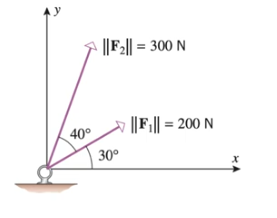
\includegraphics[width=0.5\textwidth]{1.2.1.PNG}
    \end{center}

    From the diagram, we can see that $\vec{F}_1=200\langle \cos 30\degree, \sin 30\degree\rangle = \langle 100\sqrt{3}, 100\rangle$.

    For $\vec{F}_2$, we get $\vec{F}_2=\langle 300\cos 70\degree, 300\sin 70\degree\rangle$.

    Adding them gives $\vec{F}=\langle 100\sqrt{3}+300\cos 70\degree, 100+300\sin 70\degree\rangle$.

    This approximates to $\langle 275.8,381.9\rangle$. The magnitude of this approximates to $\|\vec{F}\|\approx 471$ N.

    If we let $100\sqrt{3}+300\cos 70\degree$ be $\|\vec{F}\|\cos\theta$, then we can determine the angle. 

    When we find $\theta$ in $\cos\theta = \frac{100\sqrt{3}+300\cos 70\degree}{471}$, we get $\theta \approx 54.2\degree$.
\end{example}

\pagebreak
\begin{example}
    A 100-lb weight hangs from two wires. Find the forces (tensions) $\vec{T}_1$ and $\vec{T}_2$ in both wires and the magnitude of those tensions.
    \begin{center}
        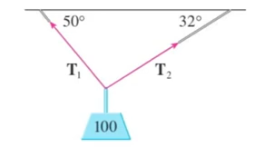
\includegraphics[width=0.5\textwidth]{1.2.2.PNG}
    \end{center}

    Note that $\vec{T}_1$ does not have an angle of $50\degree$, rather it has a degree of $130\degree$ from the point.

    Therefore, we have $\vec{T}_1=|\vec{T}_1|\langle \cos 130\degree, \sin 130\degree\rangle$.

    Note we can rewrite this with to be in the first quadrant as $|\vec{T}_1|\langle -cos 50\degree, \sin 50\degree\rangle$.

    We also have $\vec{T}_2=|\vec{T}_2|\langle \cos 32\degree, \sin 32\degree\rangle$.

    We also see that the weight of the block is $\vec{W}=100\langle 0,-1\rangle = \langle 0,-100\rangle$, so we see to balance this out, both tension forces need to equal $\langle 0,100\rangle$.

    Therefore, we see that $-|\vec{T}_1|\cos 50\degree + |\vec{T}_2|\cos 32\degree = 0$ (addition of the $\vec{i}$ components).

    We also have $|\vec{T}_1\sin 50\degree + |\vec{T}_2|\sin 32\degree = 100$ ($\vec{j}$ components).

    Solving for $|\vec{T}_1|$ and $|\vec{T}_2|$ from this gives us $85.64$ lbs and $64.91$ lbs respectively.

    Plugging these values back in gives us the tension vectors. 

    $\vec{T}_1 \approx \langle -55.05, 65.60\rangle$

    $\vec{T}_2 \approx \langle 55.05, 34.40 \rangle$
\end{example}

\section{The Dot Product}
\begin{definition}[The Dot Product]
    If $\vec{a}=\langle a_1,a_2,a_3\rangle$ and $\vec{b}=\langle b_1,b_2,b_3\rangle$, then the dot product $\vec{a}\cdot \vec{b}$ is 
    \[ \vec{a}\cdot \vec{b} = a_1b+1+a_2b_2+a_3b_3 \]
    This is called the scalar or inner product. (Note: 2-space is a similar idea)
\end{definition}

\begin{example}
    $(\vec{i}+2\vec{j}-3\vec{k})\cdot (2\vec{j}-\vec{k})$

    Using the dot product formula gives you $7$.
\end{example}

Properties of dot products:
\begin{enumerate}
    \item $\vec{a}\cdot \vec{a} = |\vec{a}|^2$
    \item $\vec{a}\cdot \vec{b} = \vec{b}\cdot \vec{a}$
    \item $\vec{a}\cdot (\vec{b}+\vec{c})=\vec{a}\cdot \vec{b}+\vec{a}\cdot \vec{c}$
    \item $(c\vec{a})\cdot \vec{b}=c(\vec{a}\cdot \vec{b})=\vec{a}\cdot (c\vec{b})$
    \item $\vec{0}\cdot \vec{a}=0$
\end{enumerate}

\begin{example}
    Prove the first property from above.

    Let $\vec{a}=\langle a_1,a_2,a_3\rangle$.

    The dot product of $\vec{a}$ and $\vec{a}$ gives us $a_1^2+a_2^2+a_3^2$.

    The magnitude of this is $\sqrt{a_1^2+a_2^2+a_3^2}^2$ which is equal to $|\vec{a}|^2$ \qed
\end{example}

\begin{example}
    Prove the third property from above.

    Let $\vec{a}=\langle a_1,a_2,a_3\rangle$, likewise for $\vec{b}$ and $\vec{c}$.

    Then when we do $\vec{a}\cdot (\vec{b}+\vec{c})$ we get 
    \begin{align*}
        \langle a_1,a_2,a_3\rangle \cdot (\langle b_1,b_2,b_3\rangle + \langle c_1,c_2,c_3\rangle)\\
        = \langle a_1,a_2,a_3\rangle \cdot \langle b_1+c_1, b_2+c_2, b_3+c_3\rangle\\
        = a_1(b_1+c_1)+a_2(b_2+c_2)+a_3(b_3+c_3)\\
        = a_1b_1+a_1c_1+a_2b_2+a_2c_2+a_3b_3+a_3c_3\\
        = (a_1b_1+a_2b_2+a_3b_3)+(a_1c_1+a_2c_2+a_3c_3)\\
        = \vec{a}\cdot \vec{b}+\vec{a}\cdot \vec{c} 
    \end{align*}\qed 
\end{example}

\begin{theorem}
    $\vec{a}\cdot \vec{b}=|\vec{a}\|\vec{b}|\cos\theta$, where $\theta$ is the angle between $\vec{a}$ and $\vec{b}$.
\end{theorem}
\begin{corollary}
    $\cos\theta = \frac{\vec{a}\cdot \vec{b}}{|\vec{a}\|\vec{b}|}$
\end{corollary}

\begin{example}
    Find the angle between $\vec{u}=\vec{i}-2\vec{j}+2\vec{k}$ and $\vec{v}=-3\vec{i}+6\vec{j}+2\vec{k}$.

    The dot product of the two gives $-11$.

    The magnitude of $\vec{u}$ is $3$ and the magnitude of $\vec{v}$ is $7$.

    We see that $\cos\theta = -\frac{11}{3\cdot 7}$, so $\theta = 2.12$ radians or $121.6\degree$.
\end{example}

Recall, $\vec{a}\cdot \vec{b}=|\vec{a}\|\vec{b}|\cos\theta$. Since $|\vec{a}\|\vec{b}|$ is always positive, the sign of the dot product is determined by $\cos\theta$.
\begin{itemize}
    \item If $\vec{a}\cdot \vec{b}>0$, then the angle is acute.
    \item If $\vec{a}\cdot \vec{b}<0$, then the angle is obtuse.
    \item If $\vec{a}\cdot \vec{b}=0$, then the vectors are orthogonal.
\end{itemize}

To determine if two vectors are parallel, the vectors have to be scalar multiples of each other.

\begin{definition}[Direction Angles]
    The direction angles $\alpha$, $\beta$, and $\gamma ([0,\pi])$ are the angles that $\vec{a}$ makes with the positive $x-$, $y-$, and $z-$ axes. Their cosines are called direction cosines.
\end{definition}
$\cos\alpha = \frac{\vec{a}\cdot \vec{i}} \implies \cos\alpha = \frac{a_1}{|\vec{a}|}$. Likewise, $\cos\beta = \frac{a_2}{|\vec{a}|}$ and $\cos\gamma = \frac{a_3}{|\vec{a}|}$.

Notice that $\cos^2\alpha + \cos^2\beta + \cos^2\gamma = 1$.

Also $\vec{a}=|\vec{a}|\langle \cos \alpha, \cos\beta, \cos\gamma \rangle$, which can be expressed as $\frac{\vec{a}}{|\vec{a}|}=\langle \cos\alpha, \cos\beta, \cos\gamma\rangle$.

So, the direction cosines form the unit vector in the direction of $\vec{a}$.

\begin{example}
    Find the direction cosines of $\vec{a}=\langle 2,-4,4\rangle$ and approximate the direction angles to the nearest degree.

    The magnitude of $\vec{a}$ is $6$.

    From the formulas, we can find that $\cos\alpha = \frac{1}{3}$, $\cos\beta = -\frac{2}{3}$, and $\cos\gamma = \frac{2}{3}$.

    Finding the angles gives us $\alpha \approx 71\degree$, $\beta \approx 132\degree$, and $\gamma \approx 48\degree$.
\end{example}

\begin{example}
    Find the angle between a diagonal of a cube and one of its edges.

    Let's call the vector from the diagonal to the edge as $\vec{d}$ and the length of the edge be $a$.

    We get $\vec{d}=\langle a,a,a\rangle$ as a result. The magnitude of $\vec{a}$ ends up being $\sqrt{3a^2}$.

    We get that $\cos\alpha = \frac{a}{\sqrt{3a^2}}=\frac{1}{\sqrt{3}}$.

    This approximates $\alpha \approx 0.955$ radians or $54.7\degree$.
\end{example}

proj$_{\vec{a}}\vec{b}$ is the vector projection of $\vec{b}$ onto $\vec{a}$

comp$_{\vec{a}}\vec{b}$ is the scalar projection of $\vec{b}$ onto $\vec{a}$ (a signed magnitude of the vector projection).

If we look at the scalar projection, comp$_{\vec{a}}\vec{b}=|\vec{b}|\cos\theta$ and remember that $\cos\theta = \frac{\vec{a}\cdot\vec{b}}{|\vec{a}\|\vec{b}|}$.
Therefore comp$_{\vec{a}}\vec{b}=\frac{\vec{a}\cdot \vec{b}}{|\vec{a}|}$.

The projection will just be the magnitude (which is the scalar projection) multiplied by the unit vector: $\frac{\vec{a}\cdot \vec{b}}{|\vec{a}|}\left(\frac{\vec{a}}{|\vec{a}|}\right)$.

This is equal to $\frac{\vec{a}\cdot \vec{b}}{|\vec{a}|^2}\vec{a}$.

\begin{example}
    Find the scalar and vector projections of $\vec{b}=\langle 1,1,2\rangle$ onto $\vec{a} = \langle -2,3,1\rangle$.

    The dot product of the vectors is $3$, the magnitude of $\vec{a}=\sqrt{14}$.

    From the formula above, the scalar projection is $\frac{3}{\sqrt{14}}$.

    The vector projection gives $\frac{3}{(\sqrt{14})^2}\langle -2,3,1\rangle$, simplifying to $\langle -\frac{3}{7},\frac{9}{14},\frac{3}{14} \rangle$.
\end{example}

Previously, you learnt work is defined as $W=F\cdot d$ (this only applies when the force is directed along the line of motion).

Now we can define work as $W=(|\vec{F}|\cos\theta)|\vec{d}|$. Moving stuff around gives $W=|\vec{F}\|\vec{D}|\cos\theta$.

Now we see that $W=\vec{F}\cdot \vec{d}$. (Work is constant which means it should result in a scalar.)

\begin{example}
    A wagon is pulled horizontally by exerting a constant force of 10 lb on the handle at an angle of $60\degree$ with the horizontal. How much work is done in moving the wagon 50 feet?

    We can easily see that the displacement vector is $\vec{d}=\langle 50,0\rangle$.

    The force vector we must divide into components, so we get $\vec{F}=10\langle \cos 60\degree, \sin 60\degree\rangle = \langle 5,5\sqrt{3}\rangle$.

    So the dot product of both vectors gives us $250$ ft-lb.
\end{example}

\section{The Cross Product}
To the interested reader that has gotten this far, review how to find the determinant of a matrix.
\ex $\begin{vmatrix}
    4&-2\\-5&-1
\end{vmatrix}$

\ex $\begin{vmatrix}
    3&-1&4\\2&-2&5\\4&-1&0
\end{vmatrix}$

Remember: when you see the straight vertical bars, you are trying to find the determinant.

Also remember 
\begin{itemize}
    \item If any two rows are the same, the determinant is zero.
    \item Interchanging two rows in a determinant multiplies the value by $-1$.
\end{itemize}

\begin{definition}[Cross Product]
    If $\vec{a}=\langle a_1,a_2,a_3\rangle$ and $\vec{b}=\langle b_1,b_2,b_3\rangle$, then the cross product of $\vec{a}$ and $\vec{b}$ is:
    \[ \vec{a}\times \vec{b}=\langle a_2b_3-a_3b_2,a_3b_1-a_1b_3,a_1b_2-a_2b_1\rangle \]
    OR 
    \[ \begin{vmatrix}
        \vec{i} & \vec{j} & \vec{k}\\
        a_1 & a_2 & a_3\\
        b_1 & b_2 & b_3
    \end{vmatrix} \]
    Notice: This is a vector.
\end{definition}

\begin{example}
    $\vec{u}=\langle 1,2,-2\rangle$ and $\vec{v}=\langle 3,0,1\rangle$. Find $\vec{u}\times \vec{v}$ and $\vec{v}\times \vec{u}$.

    First set up $\vec{u}\times \vec{v}$.

    This is $\begin{vmatrix}
        \vec{i} & \vec{j} & \vec{k}\\
        1 & 2 & -2\\
        3 & 0 &1
    \end{vmatrix}$.

    This is $\vec{i}\begin{vmatrix}
        2 & -2\\ 0 & 1
    \end{vmatrix}-\vec{j}\begin{vmatrix}
        1 & -2\\
        3 & 1
    \end{vmatrix}+\vec{k}\begin{vmatrix}
        1 & 2\\
        3& 0
    \end{vmatrix}$.

    This gives you a vector $\vec{u}\times \vec{v}=2\vec{i}-7\vec{j}-6\vec{k}$.

    Now when we set up $\vec{v}\times \vec{u}$, notice that the two rows will be interchanged. Therefore $\vec{v}\times \vec{u}=-2\vec{i}+7\vec{j}+6\vec{k}$.
\end{example}

Important: $\vec{a}\times \vec{b}$ is orthogonal to BOTH $\vec{a}$ and $\vec{b}$. (If you are asked to find a vector orthogonal to both $\vec{a}$ and $\vec{b}$, this is useful.)

Use the Right-Hand Rule to find direction. If the fingers of your right hand curl in the direction of rotation (less than $180\degree$) from $\vec{a}$ to $\vec{b}$, then your thumb points in the direction of $\vec{a}\times \vec{b}$.

Properties of the Cross Product:
\begin{enumerate}
    \item $\vec{a}\times \vec{b}=-\vec{b}\times \vec{a}$
    \item $(c\vec{a})\times \vec{b}=c(\vec{a}\times \vec{b})=\vec{a}\times (c\vec{b})$
    \item $\vec{a}\times (\vec{b}+\vec{c})=\vec{a}\times \vec{b}+\vec{a}\times \vec{c}$
    \item $(\vec{a}+\vec{b})\times \vec{c}=\vec{a}\times \vec{c}+\vec{b}\times \vec{c}$
    \item $\vec{a}\cdot (\vec{b}\times \vec{c})=(\vec{a}\times \vec{b})\cdot \vec{c}$
    \item $\vec{a}\times (\vec{b}\times \vec{c})=(\vec{a}\cdot \vec{c})\vec{b}-(\vec{a}\cdot \vec{b})\vec{c}$
\end{enumerate}

A few more important things:
\begin{itemize}
    \item $\|\vec{a}\times \vec{b}\|=\|\vec{a}\|\|\vec{b}\|\sin\theta$ (Similar to the dot product)
    \item $\vec{a}$ and $\vec{b}$ are parallel if and only if $\vec{a}\times \vec{b}=\vec{0}$. This is because $\sin\pi = 0$.
    \item The length of $\vec{a}\times \vec{b}$ is equal to the area of the parallelogram determined by $\vec{a}$ and $\vec{b}$.
\end{itemize}

\begin{example}
    Find a vector perpendicular to the plane that passes through the points $P(1,4,6)$, $Q(-2,5,-1)$, and $R(1,-1,1)$.

    We need to find $\overrightarrow{PQ}\times \overrightarrow{PR}$ to find the vector perpendicular to the plane.

    Finding $\overrightarrow{PQ}$ gives $\langle -3,1,-7\rangle$ and finding $\overrightarrow{PR}$ gives $\langle 0,-5,-5\rangle$.

    The cross product of this is $-40\vec{i}-15\vec{j}+15\vec{k}$. (All scalar multiples of this are also perpendicular.)
\end{example}

\begin{example}
    Find the area of a triangle determined by $P_1(2,2,0), P_2(-1,0,2)$, and $P_3(0,4,3)$.

    First you want to find the area of the parallelogram, then divide it by two.

    Previously, the area of the parallelogram was determined by $\|\overrightarrow{P_1P_2}\times \overrightarrow{P_1P_3}\|$.

    Do a similar process as the last example, the cross product is $\langle -10,5,-10\rangle$.

    The magnitude of this vector is $15$, so the area of the triangle is $15/2$.
\end{example}

Now the scalar triple product: we have $\vec{a}\cdot (\vec{b}\times \vec{c})$. This gives a scalar.

Note this is $\begin{vmatrix}
    a_1 & a_2 & a_3\\
    b_1 & b_2 & b_3\\
    c_1 & c_2 & c_3
\end{vmatrix}$

The absolute value of this scalar triple product gives the volume of a parallelpiped determined by $\vec{a}$, $\vec{b}$, and $\vec{c}$. (Note: absolute value, not magnitude.)

\begin{example}
    Use the scalar triple product to show that $\vec{a}=\langle 1,4,-7\rangle$, $\vec{b}=\langle 2,-1,4\rangle$, and $\vec{c}=\langle 0,-9,18\rangle$ are coplanar.

    The scalar triple product of this will give a determinant of 0. The volume of the parallelpiped therefore is 0, which means that all three vectors are coplanar (meaning on the same plane).
\end{example}

Torque measures the tendency of a body to rotate about the origin. The direction of the torque vector indicates the axis of rotation.

$\vec{\tau}=\vec{r}\times \vec{F}$ where $\vec{r}$ represents position and $\vec{F}$ represents force.

\begin{example}
    A bolt is tightened by applying a 40-N force to a 0.25 m as shown. Find the magnitude of the torque about the center of the bolt.
    \begin{center}
        
\includegraphics[width=0.5\textwidth]{1.4.1.PNG}
    \end{center}

    Remember: the $\vec{r}$ value must be in meters.

    We know that $|\vec{tau}|=|\vec{r}\|\vec{F}|\sin\theta$ (Cross Product)

    So plug in numbers to get $|\vec{\tau}| \approx 9.66$ N-m.
\end{example}

\begin{example}
    The figure shows a force of 100-N applied in the positive $z$-direction at the point $Q(1,1,1)$. Assuming the cube is free to rotate about $P(0,0,0)$, find the scalar moment (aka torque) of the force about $P$.
    \begin{center}
        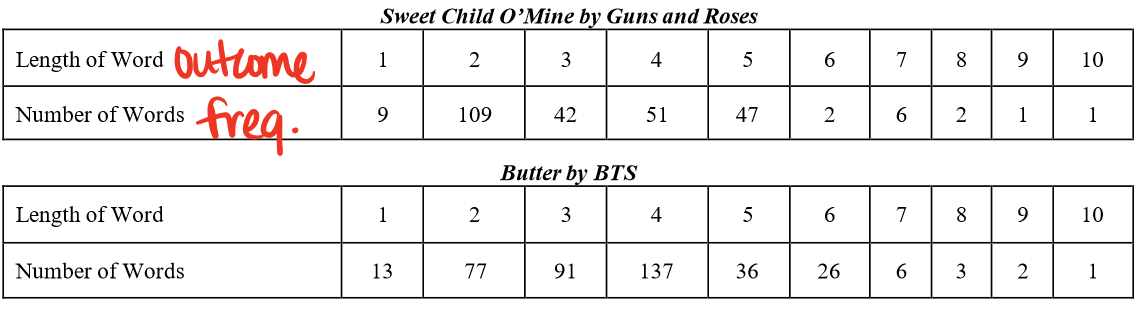
\includegraphics[width=0.5\textwidth]{1.4.2.PNG}
    \end{center}

    We know that $\vec{F}=\langle 0,0,100\rangle$ from the diagram.

    The vector $\vec{r}$ will be $\overrightarrow{PQ} = \langle 1,1,1\rangle$.

    So the cross product of the two vectors gives the torque vector.

    This vector is $\langle 100,-100,0\rangle$.
\end{example}

\section{Equations of Lines and Planes}
To write the equation of a line, you need a point and the position.

\begin{center}
    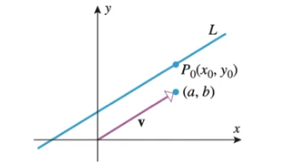
\includegraphics[width=0.5\textwidth]{1.5.E1.PNG}
\end{center}
In this figure, we know $P_0$ is a point on the line. The direction of the line is determined by a parallel vector $\vec{v}$. If $\vec{a}=\vec{P}_0P$, then $\vec{a}=t\vec{v}$.

Therefore, the vector equation of a line is $\vec{r}=\vec{r}_0+t\vec{v}$. Each value of $t$ gives a different point on the line. For $t>0$, points are to the right.

Another expression is if we let $\vec{r}=\langle x,y,z\rangle$, $\vec{r}_0=\langle x_0,y_0,z_0\rangle$, and $\vec{v}=\langle a,b,c\rangle$, then we can write this as 
\[ \langle x,y,z \rangle = \langle x_0+ta, y_0+tb, z_0+tc\rangle \]

This leads us to the parametric equation of a line. The parametric equations of a line through $(x_0,y_0,z_0)$ and parallel to the direction vector $\langle a,b,c\rangle$ are:
\[ x=x_0+at \qquad y=y_0+bt \qquad z=z_0+ct \]

\begin{example}
    Find a vector and parametric equations for the line that passes through $(4,2)$ and is parallel to $\vec{v}=\langle -1,5\rangle$. Then find 2 other points on that line.

    We have the vector $\vec{r}=\langle 4,2\rangle + t\langle -1,5\rangle$. This is the vector equation. This can also be written as $\vec{r}=(4\vec{i}+2\vec{j})+t(-\vec{i}+5\vec{j})$.
    Also this can be written as $\vec{r}=(4-t)\vec{i}+(2+5t)\vec{j}$. 

    For the parametric, we have $x=4-t$ and $y=2+5t$.

    Note: These equations are not unique. You can choose a different point or parallel vector.

    To find 2 other points, just plug in $t$ values.

    For $t=1$, we can get $x=3$, and $y=7$, so the point is $(3,7)$.
\end{example}

\begin{example}
    Find parametric equations of the line passing through $P_1(2,4,-1)$ and $P_2(5,0,7)$. Where does this line intersect the $xy$-plane?

    We have $\overrightarrow{P_1P_2}=\langle 3,-4,8\rangle$.

    We can find the parametric equations as $x=2+3t, y=4-4t$, and $z=-1+8t$ using $P_1$. (Note any scalar multiple of $\overrightarrow{P_1P_2}$ will be parallel to the line).

    This will intersect the $xy$-plane when $z=0$. So if we let $-1+8t=0$, $t=\frac{1}{8}$.

    Plugging this in $x$ and $y$ gives the point $\left(\frac{19}{8},\frac{7}{2},0\right)$ as the intersection point.
\end{example}

\pagebreak
A third representation is symmetric equations. Setting the parametric equations and solving for $t$ gives the following:
\[ t = \frac{x-x_0}{a} = \frac{y-y_0}{b} = \frac{z-z_0}{c} \]

\begin{example}
    For the last example, write the symmetric equations for the line.

    This is just $\frac{x-2}{3}=\frac{y-4}{-4}=\frac{z+1}{8}$.
\end{example}
What happens if we limit $t$? You get a line segment.

\begin{example}
    Find parametric equations for the line segment joining $P(2,4,-1)$ and $Q(5,0,7)$.

    First, $\overrightarrow{PQ}=\langle 3,-4,8\rangle$.

    The parametric equations are $x=2+3t, y=-4+4t$, and $z=-1+8t$. We have to limit $t$ though as $0\leq t\leq 1$ for this to work.

    A different representation for $\vec{r}(t)=(1-t)\vec{r}_0+t\vec{r}_1=\vec{r}_0+t(\vec{r}_1-\vec{r}_0)$.

    So for this example, this would be $(1-t)\langle 2,4,-1\rangle + t\langle 5,0,7\rangle$.
\end{example}

\begin{example}
    Consider the following lines. Are they parallel? Do they intersect?
    \[ L_1 \qquad x=1+4t \quad y=5-4t \quad z=-1+5t\]
    \[ L_2 \qquad x=2+8t \quad y=4-3t \quad z=5+t \]

    Writing these in vector form gives $L_1$ as $\langle x,y,z\rangle = \langle 1,5,-1\rangle + t\langle 4,-4,5\rangle$, and $L_2$ as $\langle x,y,z\rangle = \langle 2,4,5\rangle + t\langle 8,-3,1\rangle$.

    We can see that the $t$ terms are not scalar multiples of each other, so the lines are not parallel.

    To find intersection points, we need to see if the points of the two lines can ever equal each other.

    This means we have the equations $1+4t_1=2+8t_2$, $5-4t_1=4-3t_2$, and $-1+5t_1=5+t_2$.

    Solving for $t_1$ in this system gives us $t_1=\frac{1}{4}$ and $t_2=0$.

    This means when $t_1=\frac{1}{4}$ and $t_2=0$, then $L_1$ and $L_2$ have the same $x,y$.

    What we can see from this, is that for the last equation for $z$, they do not equal each other. That means both lines have a different $z$ value. That means the line skews because they are not parallel or intersect.
\end{example}

Unlike a line, a vector parallel to a plane is not enough information to determine a plane. Instead we need a vector perpendicular to the plane.

The equation of a plane is $\vec{n}\cdot (\vec{r}-\vec{r}_0)=0$. (This is the vector equation of a plane.)

An alternate form is $\langle a,b,c\rangle\cdot \langle x-x_0,y-y_0,z-z_0\rangle =0$. This is also $a(x-x_0)+b(y-y_0)+c(z-z_0)=0$. (This is the scalar equation of a plane).

Note that ``an equation'' means that the equation is not unique.

\pagebreak
\begin{example}
    Find an equation of the plane passing through $(3,-1,7)$ and perpendicular to the vector $\vec{n}=\langle 4,2,-5\rangle$.

    The equation is $\langle 4,2,-5\rangle \cdot \langle x-3,y+1,z-7\rangle =0$.

    This can be written as $4(x-3)+2(y+1)-5(z-7)=0$ or $4x+2y-5z+25=0$. The second equation of this is known as the linear equation.

    To graph this, we need to find 3 points (that are not co-linear). To find 3 points, you would need to come up with the intercepts, and then graph those and that gives you the plane.
\end{example}

\begin{example}
    Find an equation of the plane that passes through $P(1,3,2)$, $Q(3,-1,6)$ and $R(5,2,0)$.

    If we find the cross product of $\overrightarrow{PQ}$ and $\overrightarrow{PR}$, this will find the vector perpendicular to the plane.

    We can find that $\overrightarrow{PQ}=\langle 2,-4,4\rangle$ and $\overrightarrow{PR}=\langle 4,-1,-2\rangle$ and that $\vec{n}=\overrightarrow{PQ}\times \overrightarrow{PR}$.

    The cross product is $\langle 12,20,14\rangle$. Dividing by 2 gives us $\langle 6,10,7\rangle$, which is also perpendicular to the plane.

    So an equation of the plane is $6(x-1)+10(y-3)+7(z-2)=0$ or $6x+10y+7z=50$. (There are many ways to represent this.)
\end{example}

\begin{example}
    Consider the planes $x+y+z=1$ and $x-2y+3z=1$. Find the angle between the two planes and find symmetric equations for the line of intersection of the two planes.

    We have $\vec{n}_1=\langle 1,1,1\rangle$ and $\vec{n}_2=\langle 1,-2,3\rangle$.

    We know that $\cos\theta = \frac{\vec{n}_1\cdot \vec{n}_2}{|\vec{n}_1|\cdot |\vec{n}_2|}$.

    So plugging in numbers gives $\theta \approx 72\degree$.

    The two planes of the two normal vectors will form a parallelogram. Remember $\vec{n}_1$ and $\vec{n}_2$ are normal vectors to the plane. 

    To find symmetric equations we need a point on the line and a parallel vector.

    We will choose the point where the lines intersects the $xy$-plane ($z=0$), so $x+y=1$ and $x-2y=1$. Solving this system gives $x=1$ and $y=0$.

    Both planes have the point $(1,0,0)$. If line $L$ lies on both planes, then the line must be perpendicular to both $\vec{n}_1$ and $\vec{n}_2$.

    The cross product of the two vectors is $\langle 5,-2,-3\rangle$.

    So the symmetric equation is $\frac{x-1}{5}=\frac{y}{-2}=\frac{z}{-3}$. (There are other representations.)
\end{example}

\begin{theorem}
    The distance between a point $P(x_1,y_1,z_1)$ and plane $ax+by+cz+d=0$ is 
    \[ D=\frac{|ax_1+by_1+cz_1+d|}{\sqrt{a^2+b^2+c^2}} \]
\end{theorem}

\pagebreak
\begin{example}
    Find the distance between parallel planes $x+2y-2z=3$ and $2x+4y-4z=7$.

    We have $\vec{n}_1=\langle 1,2,-2\rangle$ and $\vec{n}_2=\langle 2,4,-4\rangle$.

    We can see that the point $(3,0,0)$ is on the first plane (letting $y=z=0$).

    For the second equation we have $2x+4y-4z-7=0$.

    From this, we have all the values needed now.

    Plugging into the distance formula gives $\frac{1}{6}$.
\end{example}

\begin{example}
    From a previous example, you found the lines are skew. Find the distance between them.
    \[ L_1 \qquad x=1+4t \quad y=5-4t \quad z=-1+5t\]
    \[ L_2 \qquad x=2+8t \quad y=4-3t \quad z=5+t \]

    First find a point on $L_1$. We get a point $(1,5,-1)$ (when $t=0$).

    We need to find a plane through $L_2$ and need a point and a perpendicular vector.

    We know a point would be $(2,4,5)$. To find the perpendicular vector, we need to find a cross product of $\vec{L}_1\times \vec{L}_2$.

    The cross product is $\langle 11,-36,20\rangle$. So the equation of the plane is $11(x-2)-36(y-4)+20(z-5)=0$.

    This can be written as $x-36y+20z+22=0$.

    Now we can find the distance since we have the plane and the point. 

    The distance is roughly $D\approx 3.918$ units.
\end{example}

\section{Cylinders and Quadric Surfaces}
\begin{definition}
    A cylinder is a surface that consists of all lines parallel to a given line and passing through a given plane curve (i.e - in 3 space, the equation only has 2 variables).
\end{definition}

For example, sketching $z=x^2$ in 3-space. This is essentialy a parabola on the $xz$-plane along a parallel line, and it will look like a piece of paper being in the process of being folded.

\ex Sketch $y^2+z^2=1$ in 3-space.

\begin{definition}
    A quadric surface is the graph of a second-degree equation in 3 variables 
    \[ Ax^2+By^2+Cz^2+Dxy+Eyz+Fxz+Gx+Hy+Iz+J =0 \]
\end{definition}

\ex Graph $z=x^2+y^2$. (Hint $z\geq 0$.)

There are 6 different quadric surfaces.

First, the ellipsoid has the general equation $\frac{x^2}{a^2}+\frac{y^2}{b^2}+\frac{z^2}{c^2}=1$.
The intercepts of this are $(0,0\pm c)$, $(0\pm b,0)$. and $(\pm a,0,0)$. For the traces, we can see that if we let $x$, $y$, or $z$ be a number, they will give ellipses. The shape of this looks like a football (American).

Next, the cone has the general equation $\frac{z^2}{c^2}=\frac{x^2}{a^2}+\frac{y^2}{b^2}$. The axis is that $\frac{z^2}{c^2}$ term, but it can be $y^2$ or $z^2$.
This has one intercept, $(0,0,0)$. The traces are $z$ is some number, it gives an ellipse, if $x$ or $y$ is some number, you get a hyperbola.

Next, the elliptic paraboloid has the equation $\frac{z}{c}=\frac{x^2}{a^2}+\frac{y^2}{b^2}$. Likewise with the cone, the $\frac{z}{c}$ term just tells you what axis (it can be $x$ or $y$.)
The intercept is the same as the cone, $(0,0,0)$. For the traces, $z$ gives an ellipse, and $x$ and $y$ gives parabolas.

Next the hyperboloid of one sheet. The equation is $\frac{x^2}{a^2}+\frac{y^2}{b^2}-\frac{z^2}{c^2}=1$. (The term with a minus is the axis.)
You have to find the intercept for this one. $z$ gives an ellipse, and $x$ and $y$ gives hyperbolas.

Next, hyperboliods of 2 sheets. The equation is $-\frac{x^2}{a^2}-\frac{y^2}{b^2}+\frac{z^2}{c^2}=1$. (The term with the plus is the axis.)
You have to find the intercept, and $z$ gives an ellipse ($z>c$), and $x$ and $y$ gives ellipses.

Lastly, the hyperbolic paraboloid. The formula is $\frac{z}{c}=\frac{x^2}{a^2}-\frac{y^2}{b^2}$. You have to find the intercept. $x$ and $y$ gives parabolas and $z$ gives a hyperbola. (This should kind of look like a saddle (on a horse).)

\begin{example}
    Let's look at $y^2=x^2+\frac{z^2}{4}$.

    The intercept is $(0,0,0)$.

    We can assume that $y$ is the axis we are drawing on. 

    When we look at the traces, they all give ellipses.
    For example, $y=1$ gives $1=x^2+\frac{z^2}{4}$, $y=2$ gives $4=x^2+\frac{z^2}{4}$ or $1=\frac{x^2}{4}+\frac{z^2}{16}$.

    When we let $x=0$, then we can get $y^2=\frac{z^2}{4}$, which gives $\pm y = \pm \frac{z}{2}$, which is two perpendicular lines essentially.

    This is an elliptic cone.
\end{example}

\begin{example}
    Let's look at $4x^2+4y^2+z^2+8y-4z=-4$.

    Completing the square gives $x^2+(y+1)^2+\frac{(z-2)^2}{4}=1$.

    The intercepts are $(0,0,2)$, $(0,-1,0)$ as the two intercepts, (there are no $x$-intercepts.) From what we also see, we can see the center of the graph should be $(0,-1,2)$.

    Hopefully, you can see that all the traces are ellipses.

    Cool! We get an ellipsoid.
\end{example}

\begin{example}
    Lastly, graph $z=\frac{y^2}{4}-\frac{x^2}{9}$.

    Starting with intercepts, we get $(0,0,0)$ as the only intercept.

    For our traces, $x$ and $y$ give parabolas, and $z$ gives a hyperbola.

    This gives a hyperbolic paraboloid.
\end{example}

\pagebreak
For a brief review on conic sections: the following.

Circles: A circle is the set of all points in the plane equidistant from a fixed point. The standard equation is $(x-h)^2+(y-k)^2=r^2$, where $(h,k)$ is the center, and $r$ is the radius.

Ellipses: An ellipse is the set of all points in the plane the sum of whose distances from two fixed points (the foci) is constant. The standard equation is $\frac{(x-h)^2}{a^2}+\frac{(y-k)^2}{b^2}=1$. 
If $a>b$, we get the foci as $(h\pm c,k)$, and if $b>a$, we get the foci as $(h,k\pm c)$. For both of these, the center will be $(h,k)$, and the vertices are the endpoints of the major axis. Use $c$ to find the coordinates of each focus. The foci are located on the major axis and are each $c$ units away from the center.
If $a=b$, then the ellipse is just a circle, and $a$ and $b$ will equal $r$. The foci of a circle are located at the same point - the center. Eccentricity of an ellipse is $\frac{c}{a}$. (For a circle $e=0$.)

Hyperbolas: A hyperbola is the set of all points in the plane the difference of whose distances from two fixed points (the foci) is constant. The standard equation are the following:
\begin{itemize}
    \item For hyperbolas that open left and right: $\frac{(x-h)^2}{a^2}-\frac{(y-k)^2}{b^2}=1$, the foci will be $(h\pm c,k)$
    \item For hypberolas that open up and down: $\frac{(y-k)^2}{b^2}-\frac{(x-h)^2}{a^2}=1$, the foci will be $(h,k\pm c)$
\end{itemize}
The center is $(h,k)$ for both and the vertices are the turning points of the brances of the hyperbola. Use $a$ and $b$ to create the central rectangle around the center of the hyperbola. The diagonals of this rectangle form the asymptotes. 
The equation for the asymptotes are $y-k=\pm \frac{b}{a}(x-h)$. Use the value $c=\sqrt{a^2+b^2}$, to find the coordinates of each focus. The branches of a hyperbola will always bend towards the foci and away from the center.

Parabolas: A parabola is the set of all points in the plane equidistant from a fixed line (the directrix) and a fixed point (the focus).
The graph of a parabola will always bend towards its focus and away from its directrix. The coordinates of the vertex are $(h,k)$, the distance from the vertex to both the focus and directrix is given by $|p|$.
For equation for a parabola that opens up and down is $(x-h)^2=4p(y-k)$, and for one that opens left or right it is $(y-k)^2=4p(x-h)$. If $p>0$, the parabola either opens up or right, and for $p<0$, the opposite happens.
\end{document}